\documentclass{standalone}
\usepackage{amsmath}
\usepackage{tikz}
\usetikzlibrary{arrows,matrix,positioning}
\begin{document}
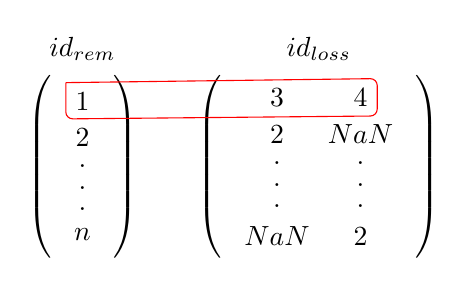
\begin{tikzpicture}


\matrix [matrix of math nodes,left delimiter=(,right delimiter=)] at (-1.5,-5) (m1)
{
    1  \\               
        2  \\               
        .  \\           
        . \\    
        . \\    
        n \\
};  
\draw (-1.5,-3.5) node{$id_{rem}$} ; 

\matrix [matrix of math nodes,left delimiter=(,right delimiter=)] at (1.5,-5) (m2)
{
    3 &4  \\               
        2 &NaN  \\               
        . &.  \\           
        . &. \\    
        . &. \\    
        NaN &2 \\
};  
\draw (1.5,-3.5) node{$id_{loss}$} ; 


% Red rectangle
\draw[color=red,rounded corners=2.5pt] (m1-1-1.north west) -- (m2-1-2.north east) -- (m2-1-2.south east) -- (m1-2-1.north west) -- (m1-1-1.north west);



% -------------------------------------------



\end{tikzpicture}
\end{document}

